\documentclass{standalone}
\usepackage{tikz}
\usetikzlibrary{patterns, positioning}
\usepackage[sfdefault]{ClearSans} %% option 'sfdefault' activates Clear Sans as the default text font
\usepackage[T1]{fontenc}

\begin{document}
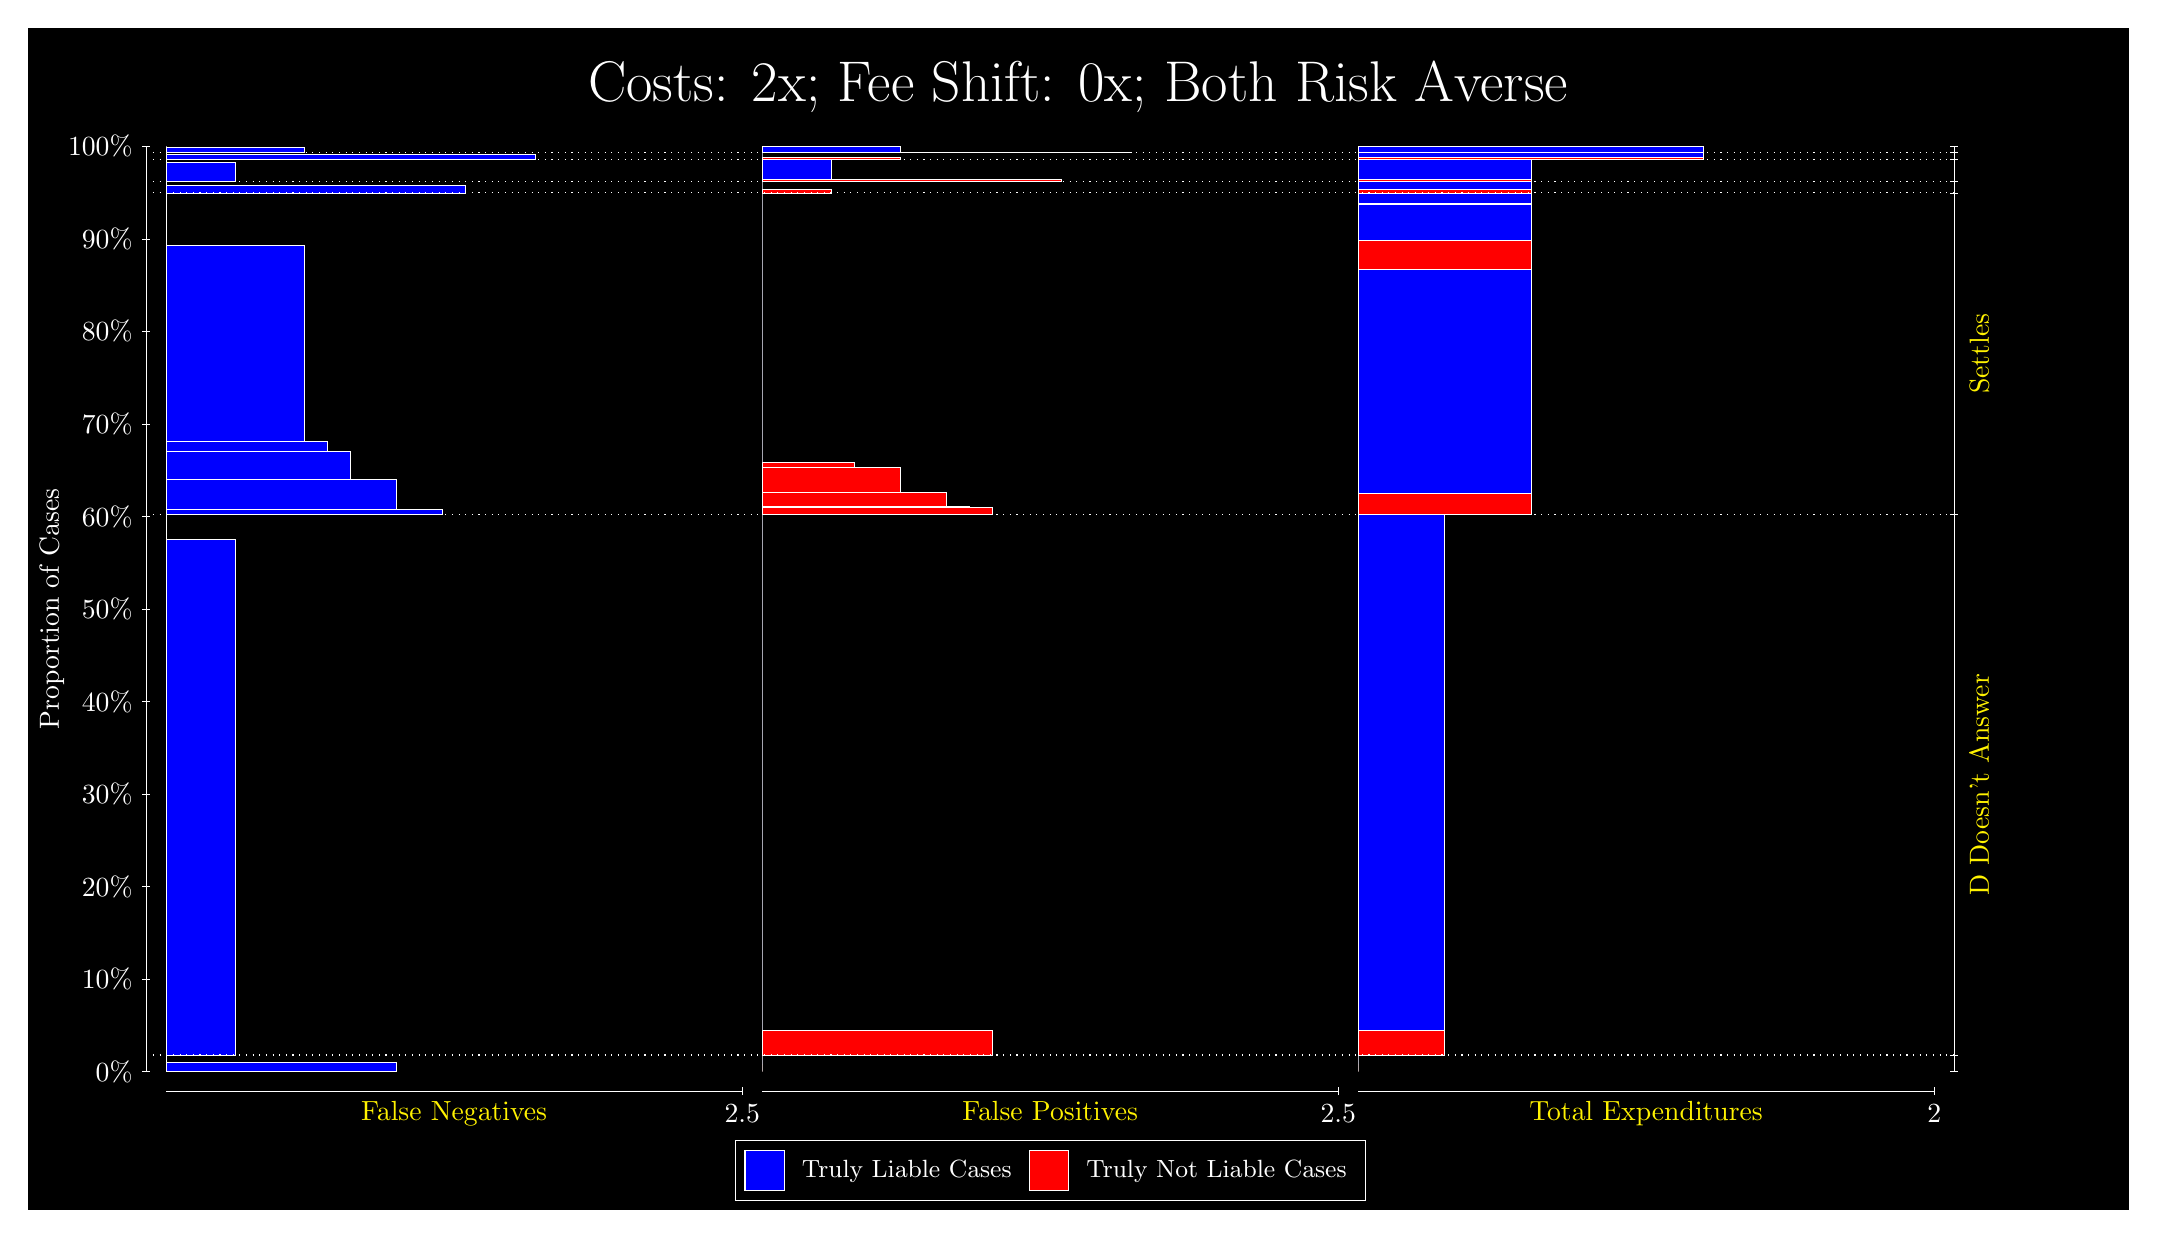
\begin{tikzpicture}
\draw[fill=black] (0,0) rectangle (26.667,15);
\draw[text=white] (0,13.5) rectangle (26.667,15) node[midway] {\huge Costs: 2x; Fee Shift: 0x; Both Risk Averse};
\draw[white, very thin] (1.5,1.75) -- (1.5,13.5);
\node[rotate=90, text=white, anchor=center] at (0.3, 7.625) {Proportion of Cases};
\draw[white, very thin] (1.45,1.75) -- (1.55,1.75);
\node[text=white, anchor=east] at (1.45, 1.75) {0\%};
\draw[white, very thin] (1.45,2.925) -- (1.55,2.925);
\node[text=white, anchor=east] at (1.45, 2.925) {10\%};
\draw[white, very thin] (1.45,4.1) -- (1.55,4.1);
\node[text=white, anchor=east] at (1.45, 4.1) {20\%};
\draw[white, very thin] (1.45,5.275) -- (1.55,5.275);
\node[text=white, anchor=east] at (1.45, 5.275) {30\%};
\draw[white, very thin] (1.45,6.45) -- (1.55,6.45);
\node[text=white, anchor=east] at (1.45, 6.45) {40\%};
\draw[white, very thin] (1.45,7.625) -- (1.55,7.625);
\node[text=white, anchor=east] at (1.45, 7.625) {50\%};
\draw[white, very thin] (1.45,8.8) -- (1.55,8.8);
\node[text=white, anchor=east] at (1.45, 8.8) {60\%};
\draw[white, very thin] (1.45,9.975) -- (1.55,9.975);
\node[text=white, anchor=east] at (1.45, 9.975) {70\%};
\draw[white, very thin] (1.45,11.15) -- (1.55,11.15);
\node[text=white, anchor=east] at (1.45, 11.15) {80\%};
\draw[white, very thin] (1.45,12.325) -- (1.55,12.325);
\node[text=white, anchor=east] at (1.45, 12.325) {90\%};
\draw[white, very thin] (1.45,13.5) -- (1.55,13.5);
\node[text=white, anchor=east] at (1.45, 13.5) {100\%};

\draw[white, very thin] (24.457,1.75) -- (24.457,13.5);
\draw[white, very thin] (24.407,1.75) -- (24.507,1.75);
\node[anchor=west] at (24.407, 1.75) {};
\draw[white, very thin] (24.407,1.9596) -- (24.507,1.9596);
\node[anchor=west] at (24.407, 1.9596) {};
\draw[white, very thin] (24.407,8.8243) -- (24.507,8.8243);
\node[anchor=west] at (24.407, 8.8243) {};
\draw[white, very thin] (24.407,12.909) -- (24.507,12.909);
\node[anchor=west] at (24.407, 12.909) {};
\draw[white, very thin] (24.407,13.052) -- (24.507,13.052);
\node[anchor=west] at (24.407, 13.052) {};
\draw[white, very thin] (24.407,13.334) -- (24.507,13.334);
\node[anchor=west] at (24.407, 13.334) {};
\draw[white, very thin] (24.407,13.421) -- (24.507,13.421);
\node[anchor=west] at (24.407, 13.421) {};
\draw[white, very thin] (24.407,13.5) -- (24.507,13.5);
\node[anchor=west] at (24.407, 13.5) {};

\draw[white, very thin, fill=blue] (1.75,1.75) rectangle (4.6775,1.8668);
\draw[white, very thin, fill=red] (1.75,1.8668) rectangle (1.75,1.9596);
\draw[white, very thin, fill=blue] (1.75,1.9596) rectangle (2.6283,8.5097);
\draw[white, very thin, fill=red] (1.75,8.5097) rectangle (1.75,8.8243);
\draw[white, very thin, fill=blue] (1.75,8.8243) rectangle (5.2631,8.8916);
\draw[white, very thin, fill=blue] (1.75,8.8916) rectangle (4.9703,8.8951);
\draw[white, very thin, fill=blue] (1.75,8.8951) rectangle (4.6775,9.2719);
\draw[white, very thin, fill=blue] (1.75,9.2719) rectangle (4.092,9.6255);
\draw[white, very thin, fill=blue] (1.75,9.6255) rectangle (3.7993,9.753);
\draw[white, very thin, fill=blue] (1.75,9.753) rectangle (3.5065,12.248);
\draw[white, very thin, fill=red] (1.75,12.248) rectangle (1.75,12.909);
\draw[white, very thin, fill=blue] (1.75,12.909) rectangle (5.5558,13.009);
\draw[white, very thin, fill=red] (1.75,13.009) rectangle (1.75,13.052);
\draw[white, very thin, fill=blue] (1.75,13.052) rectangle (2.6283,13.302);
\draw[white, very thin, fill=red] (1.75,13.302) rectangle (1.75,13.334);
\draw[white, very thin, fill=blue] (1.75,13.334) rectangle (6.4341,13.397);
\draw[white, very thin, fill=red] (1.75,13.397) rectangle (1.75,13.421);
\draw[white, very thin, fill=blue] (1.75,13.421) rectangle (3.5065,13.493);
\draw[white, very thin, fill=red] (1.75,13.493) rectangle (1.75,13.5);
\draw[white, very thin, fill=red] (9.3189,1.75) rectangle (9.3189,1.8428);
\draw[white, very thin, fill=blue] (9.3189,1.8428) rectangle (9.3189,1.9596);
\draw[white, very thin, fill=red] (9.3189,1.9596) rectangle (12.246,2.2741);
\draw[white, very thin, fill=blue] (9.3189,2.2741) rectangle (9.3189,8.8243);
\draw[white, very thin, fill=red] (9.3189,8.8243) rectangle (12.246,8.9096);
\draw[white, very thin, fill=red] (9.3189,8.9096) rectangle (11.954,8.9322);
\draw[white, very thin, fill=red] (9.3189,8.9322) rectangle (11.661,9.1103);
\draw[white, very thin, fill=red] (9.3189,9.1103) rectangle (11.075,9.4226);
\draw[white, very thin, fill=red] (9.3189,9.4226) rectangle (10.783,9.4249);
\draw[white, very thin, fill=red] (9.3189,9.4249) rectangle (10.49,9.4855);
\draw[white, very thin, fill=blue] (9.3189,9.4855) rectangle (9.3189,12.909);
\draw[white, very thin, fill=red] (9.3189,12.909) rectangle (10.197,12.952);
\draw[white, very thin, fill=blue] (9.3189,12.952) rectangle (9.3189,13.052);
\draw[white, very thin, fill=red] (9.3189,13.052) rectangle (13.125,13.084);
\draw[white, very thin, fill=blue] (9.3189,13.084) rectangle (10.197,13.334);
\draw[white, very thin, fill=red] (9.3189,13.334) rectangle (11.075,13.358);
\draw[white, very thin, fill=blue] (9.3189,13.358) rectangle (9.3189,13.421);
\draw[white, very thin, fill=red] (9.3189,13.421) rectangle (14.003,13.428);
\draw[white, very thin, fill=blue] (9.3189,13.428) rectangle (11.075,13.5);
\draw[white, very thin, fill=red] (16.888,1.75) rectangle (16.888,1.8428);
\draw[white, very thin, fill=blue] (16.888,1.8428) rectangle (16.888,1.9596);
\draw[white, very thin, fill=red] (16.888,1.9596) rectangle (17.986,2.2741);
\draw[white, very thin, fill=blue] (16.888,2.2741) rectangle (17.986,8.8243);
\draw[white, very thin, fill=red] (16.888,8.8243) rectangle (19.083,9.0877);
\draw[white, very thin, fill=blue] (16.888,9.0877) rectangle (19.083,11.936);
\draw[white, very thin, fill=red] (16.888,11.936) rectangle (19.083,12.311);
\draw[white, very thin, fill=blue] (16.888,12.311) rectangle (19.083,12.759);
\draw[white, very thin, fill=red] (16.888,12.759) rectangle (19.083,12.782);
\draw[white, very thin, fill=blue] (16.888,12.782) rectangle (19.083,12.909);
\draw[white, very thin, fill=red] (16.888,12.909) rectangle (19.083,12.952);
\draw[white, very thin, fill=blue] (16.888,12.952) rectangle (19.083,13.052);
\draw[white, very thin, fill=red] (16.888,13.052) rectangle (19.083,13.084);
\draw[white, very thin, fill=blue] (16.888,13.084) rectangle (19.083,13.334);
\draw[white, very thin, fill=red] (16.888,13.334) rectangle (21.279,13.358);
\draw[white, very thin, fill=blue] (16.888,13.358) rectangle (21.279,13.421);
\draw[white, very thin, fill=red] (16.888,13.421) rectangle (21.279,13.428);
\draw[white, very thin, fill=blue] (16.888,13.428) rectangle (21.279,13.5);
\draw[white, dotted] (1.5,1.9596) -- (24.457,1.9596);
\draw[white, dotted] (1.5,8.8243) -- (24.457,8.8243);
\draw[white, dotted] (1.5,12.909) -- (24.457,12.909);
\draw[white, dotted] (1.5,13.052) -- (24.457,13.052);
\draw[white, dotted] (1.5,13.334) -- (24.457,13.334);
\draw[white, dotted] (1.5,13.421) -- (24.457,13.421);
\draw[white, very thin] (1.75,1.5) -- (9.0689,1.5);
\node[text=yellow, anchor=north] at (5.4094, 1.5) {False Negatives};
\draw[white, very thin] (9.0689,1.45) -- (9.0689,1.55);
\node[text=white, anchor=north] at (9.0689, 1.45) {2.5};

\draw[white, very thin] (9.3189,1.5) -- (16.638,1.5);
\node[text=yellow, anchor=north] at (12.978, 1.5) {False Positives};
\draw[white, very thin] (16.638,1.45) -- (16.638,1.55);
\node[text=white, anchor=north] at (16.638, 1.45) {2.5};

\draw[white, very thin] (16.888,1.5) -- (24.207,1.5);
\node[text=yellow, anchor=north] at (20.547, 1.5) {Total Expenditures};
\draw[white, very thin] (24.207,1.45) -- (24.207,1.55);
\node[text=white, anchor=north] at (24.207, 1.45) {2};


\node[text=yellow, centered, rotate=90] at (24.777, 5.3919) {D Doesn't Answer};
\node[text=yellow, centered, rotate=90] at (24.777, 10.867) {Settles};





\draw (12.978300999999998,1.5) node[draw=none] (baseCoordinate) {};
\begin{scope}[align=center]
        \matrix[scale=0.5, draw=white, below=0.5cm of baseCoordinate, nodes={draw}, column sep=0.1cm]{
            \node[rectangle, draw, minimum width=0.5cm, minimum height=0.5cm, fill=blue] {}; &
            \node[draw=none, font=\small, text=white] (B) {Truly Liable Cases}; &
            \node[rectangle, draw, minimum width=0.5cm, minimum height=0.5cm, fill=red] {}; &
            \node[draw=none, font=\small, text=white] (B) {Truly Not Liable Cases}; \\
            };
\end{scope}

\end{tikzpicture}
\end{document}